\section{Task definition}
\label{sec:task}

We define melody transcription as the task of converting a musical audio recording into a \emph{monophonic} (non-overlapping) sequence of \emph{notes} which constitute its melody.\footnote{Melody is difficult to precisely define---here we adopt an implicit definition based on a dataset of crowdsourced melody annotations.} Given a musical audio recording $\bm{a}$ of length $T$, our task is to 
%generate 
uncover 
the sequence of $N$ notes~${\bm{y} = y_1,\dots,y_N}$ that constitute the melody of $\bm{a}$.  For many MIR tasks, including transcription, it can be convenient to work with \emph{features} of audio ${\bm{X} = \texttt{Featurize}(\bm{a})}$, rather than the raw waveform $\bm{a}$. 
Hence, a melody transcription algorithm is a procedure that maps featurized audio to notes, i.e.~${\bm{y} = \texttt{Transcribe}(\bm{X})}$. 

\begin{figure}
    \centering
    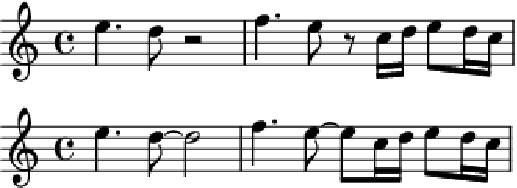
\includegraphics[width=8.1cm]{figs/heuristic_offsets.pdf}
    \caption{
The same note onsets engraved with ground truth~(top) vs. heuristic~(bottom) offsets. 
We argue that onset prediction suffices for producing melody transcriptions that are both recognizable and readable. 
}
 \label{fig:heuristic_offsets}
\end{figure}

Canonically, a musical note consists of an onset time, a musical pitch, and an offset time. 
However, in this work  
%(and as in~\cite{laaksonen2014automatic}) 
we disregard offsets and define a note to be a pair ${y_i = (t_i,n_i)}$ consisting of an onset time~${t_i \in [0,T)}$ and discrete musical pitch~${n_i \in \{\text{A0},\dots,\text{C8}\}}$.
We ignore offsets for three reasons. 
First, accurate offsets have been found to be considerably less important for human perception of transcription quality compared to accurate onsets~\cite{ycart2020investigating}. 
Second, in our dataset,
a heuristically-determined offset is identical to the ground truth offset for $89\%$ of notes.\footnote{The heuristic we adopt sets the offset of one note equal to the onset of the next, i.e., it assumes the melody is legato.}
Finally, we argue intuitively that onsets and pitches suffice for both recognizing and reading melodies---see~\Cref{fig:heuristic_offsets} for an example.

Formally, a musical audio recording of length~$T$ seconds sampled at rate~$f_s$ is a vector~${\bm{a} \in \mathbb{R}^{Tf_s}}$. 
A featurization of audio ${\bm{X} \in \mathbb{R}^{Tf_k \times d}}$ is a matrix of $d$-dimensional features of audio, sampled uniformly at some rate ${f_k \ll f_s}$ (for example, $\bm{X}$ could be a spectrogram).
Intuitively, the function ${\texttt{Featurize} : \mathbb{R}^{Tf_s} \to \mathbb{R}^{Tf_k \times d}}$ defined by ${\bm{a} \mapsto \bm{X}}$ maps 
%scalar audio samples 
raw audio 
to a feature representation more conducive to learning. 
A melody of length $N$ is an (ordered) sequence of notes 
% CHRIS: Should this be raised to the N? JOHN: nope, \bm{y} \in \mathcal{N}^N but y_1,\dots,y_N \in \mathcal{N}
${\bm{y} = y_1,\dots,y_N \in \mathbb{Y}}$, 
consisting of onset-pitch pairs ${y_i = (t_i,n_i)}$ where ${t_i < t_j}$ if ${i < j}$. Given a featurization $\bm{X}$, the melody transcription task is to construct a transcription algorithm ${\texttt{Transcribe} : \mathbb{R}^{Tf_k \times d} \to \mathbb{Y}^N}$ such that ${\bm{X} \mapsto \bm{y}}$.


%Hence, 
%\begin{gather*}
%    %\bm{a} &= a_1, \ldots, a_S, \text{where}~S %= Tf_s \\
%    \bm{y} = y_1, \ldots, y_N, \\
%    \text{where}~y_i = (t_i, n_i), t_i \leq T, %\text{and}~n_i \in \{\text{A0}, \ldots, %\text{C8}\}.
%\end{gather*}
%\todo{Remove high-dimensionality quip, replace with specifics (spectrograms)... for MIR tasks, often better to work with features rather than raw audio...}
%\john{Not sure high-dimensionality is the right motivation here}

%To handle the high dimensionality of audio, transcription algorithms typically extract features $\bm{X}$ (a matrix) from audio, which are sampled at ${f_k \ll f_s}$:
%\begin{gather*}
%    \text{Extract}(\bm{a}) = \bm{X} = \bm{x}_1, %\ldots, \bm{x}_M, \\ 
%    \text{where}~M = Tf_k, \text{and}~\bm{x}_i %\in \mathbb{R}^d.
%\end{gather*}

\subsection{Evaluation}
\label{sec:eval}

% CHRIS: This maps cleanly onto our contributions (standardized evaluation and new datasets), but may be too snarky for paragraph 2
%Finally, we argue that a historical focus on the important but disparate task of melody \emph{extraction}---detecting the time-varying fundamental frequency of the melody as opposed to its discrete notes---has led to a lack of work on transcription and systemic issues in evaluation.
% \john{Leading with an MIR implementation of F1 is a little confusing, especially since it is not typically applied to this task (you are defining the task, right?)}
% CHRIS: Reworked to clarify that this is a departure from melody extraction

%\john{Maybe lead with why we need to invent our own metrics?}
To evaluate a melody transcription method $\texttt{Transcribe}$, 
we adopt a standard metric commonly used for evaluation in polyphonic music transcription tasks, namely,  ``onset-only notewise F-measure''~\cite{ycart2020investigating}. 
This metric scores an estimated transcript $\texttt{Transcribe}(\bm{X})$ by first matching its note onsets to those in the reference $\bm{y}$ with $50$ms of tolerance, and then computes a standard \fone{} score where an estimated note is treated as correct if it is the same pitch as its matched reference note. 
% \begin{equation*}
%      \text{\fone} : f(\bm{X}), y \mapsto [0, 1].
% \end{equation*}
This ``notewise'' metric represents a departure from the ``frame-based'' metrics typically used to evaluate melody extraction algorithms---Ycart~et~al.\ demonstrate in~\cite{ycart2020investigating} that this particular notewise metric correlates more strongly with human perception of transcription quality than any other common metric, including frame-based ones.

We make a slight modification to this notewise metric 
%to make it more appropriate for 
specific to 
the melody transcription setting: an estimate $\texttt{Transcribe}(\bm{X})$ may receive full credit if it is off by a fixed octave shift but otherwise identical to the reference. 
In downstream settings, melody transcriptions are likely to be used in an octave-invariant fashion, e.g.,~they may be shifted to read more comfortably in treble clef, or performed by singers with different vocal ranges. 
% Previous evaluations for melody extraction gave full credit for estimates with the right pitch class, ignoring octaves entirely (see~\cite{poliner2007melody} for a summary). 
% However we argue that this is overly permissive, as \emph{relative} octave information preserves intervals between notes, and thus may be critical to the identity of a melody. 
Hence, we modify the evaluation criteria by simply taking the highest score over octave shifted versions of the estimate:
\begin{equation*}
    \max_{\sigma \in \mathbb{Z}} \texttt{\fone}(\texttt{OctaveShift}(\texttt{Transcribe}(\bm{X}), \sigma), \mathbf{y}).
\end{equation*}
Henceforth, we refer to this octave-invariant metric as \fone. 